\documentclass[12pt,letterpaper]{article}
\oddsidemargin 0in
\evensidemargin 0in
\textwidth 6.5in
\topmargin -0.5in
\textheight 9.0in
\usepackage{hyperref}
\usepackage{mathptmx}
\usepackage{caption}
\usepackage{comment}

\usepackage[ruled,linesnumbered,vlined]{algorithm2e}
\SetNlSty{textbf}{}{:}

\usepackage{amsmath}

\usepackage{graphicx}
\usepackage{float}	% for fixing image position 

\usepackage{natbib} % for references
\usepackage[usenames,dvipsnames]{xcolor}
\newcommand{\blue}[1]{\textcolor{RoyalBlue}{#1}}
\newcommand{\fillme}[1]{\blue{\texttt{[Insert #1]}}}
\newcommand{\instructions}[1]{\blue{\textit{#1}}}


\begin{document}

\title{An Unsupervised Approach to Word Sense Disambiguation \\ \Large{(CS446 Class Project)}}
\author{Haoruo Peng (hpeng7@illinois.edu) \and Shyam Upadhyay (upadhya3@illinois.edu)}
\maketitle
\begin{abstract}
We investigate the task of word sense disambiguation using an unsupervised approach. Word sense disambiguation is the task of identifying the correct sense for a word which can possibly admit multiple senses. We use the Semeval-2007 dataset to evaluate the performance of our system. We use a graph based approach to disambiguate senses; the underlying assumption is that the sense of the neighboring words can assist in inferring the sense of the target word. In this respect, the senses are learnt in a joint-manner. Using appropriate weights in the graph constructed for all possible senses, we can use the graph to obtain measures of centrality, which can guide the sense-disambiguation.
%\instructions{Very briefly, summarize your task, your model and your main results}
\end{abstract}


\section{Introduction} 
\label{sec:introduction}
In natural language, a word may be associated with possibly multiple meanings, depending on the context in which the word occurs. For instance, the word pen has the following senses according to Wordnet~\cite{wordnet}:
\begin{description}
\item [pen] : a writing implement with a point from which ink flows
\item [pen] : an enclosure for confining livestock
\item [pen] : a female swan
\end{description}
In linguistic parlance such words are called polysemous. \emph{Word sense disambiguation}(WSD) is the problem of determining the correct sense of a polysemous word in a given sentence or document. Features of the document (like neighboring words, earlier usage of the same word etc.) help in determining the sense. For example, determining the correct sense of the word ``pen" in the following passage:
\begin{verbatim}
Little John was looking for his toy box. Finally he found it. 
The box was in the pen. John was very happy.
\end{verbatim}
WSD can be viewed as a multi-class classification problem, where each word admits several possible senses and the task is to identify the correct sense of a given word given its context and knowledge sources. The inherent difficulty of WSD is evident from the fact that the target classes change for each word in the lexicon. In this respect, WSD involves training $n$ different classifiers, one for each word in a lexicon of size $n$. 
%\subsection{Motivation}
WSD is a intermediate step in language processing, like part-of-speech tagging or shallow parsing. It is a key component for natural language processing systems which involves semantic interpretation of text. Tasks such as machine translation, information retrieval, data mining, web data analysis can greatly benefit from text disambiguation tools. 


\section{Background}
\label{sec:background}
%\instructions{Summarize and discuss related work that you are building on: this requires you to find, read and cite a few research papers. This is also something you can get started on as soon as you have settled on a task.} 

The task of WSD was first described by Warren Weaver in 1949. He encountered the problem while working on machine translation. In those days, researchers such as Bar-Hillel felt that WSD could not be solved without modelling world knowledge. WSD has been described as an AI-complete problem~\cite{mallery1988thinking}, which means that it is computationally as hard as solving central artificial intelligence problems like the Turing test. Until 1970s, semantic interpretation systems used rule based patterns to resolve the senses, which were hand-coded and hence error prone. It was only in the 1980s, when lexical resources like Oxford Advanced Learner's Dictionary of Current English (OALD) became available and dictionary-based methods were used for the first time. 

Today, significant progress has been made in WSD and researchers have achieved sufficiently high levels of accuracy on a variety of word types and ambiguities. A rich variety of techniques have been used, from dictionary-based methods~\cite{mihalcea2007using} that use the knowledge encoded in lexical resources, to supervised machine learning methods~\cite{manning1999foundations} in which a classifier is trained for each distinct word on a corpus of manually sense-annotated examples, to completely unsupervised methods~\cite{yarowsky1995unsupervised} that cluster occurrences of words, thereby inducing word senses.

Supervised learning approaches have been remarkably successful for performing word sense disambiguation. Instance-based learning and SVM approaches have proven to be the best systems in several competition. The only issue with supervised approaches is the lack of sense-tagged data which poses a severe bottleneck. 

To address this problem, researchers have resorted to semi-supervised learning algorithms. The Yarowsky algorithm~\cite{yarowsky1995unsupervised} was an early example of such an algorithm. It uses the `One sense per collocation' and the `One sense per discourse' properties of human languages for word sense disambiguation. From observation, words tend to exhibit only one sense in most given discourse and in a given collocation. The common motif in approaches like ~\cite{yarowsky1995unsupervised},~\cite{le2008semi} is that they allows both labeled and unlabeled data. Training involve iteratively labeling the unlabeled data using an initial seeding labeled set. The seed labeled data is used to learn a classifier which is used to assign labels to unlabeled data, which is merged with the initial seed data to obtain a larger dataset for the next iteration. Finally, the classifier is learned from the extended labelled dataset.
More recently, researchers~\cite{Ng} have leveraged word alignment information from parallel corporas to aid in obtaining coarse grained senses. The aim of word-alignment task is to align a word in a given sentence to its translated counterpart in another sentence in a different language. Unlike sense-tagged datasets, good quality parallel corpora are readily available. 

%The bootstrapping approach starts from a small amount of seed data for each word: either manually tagged training examples or a small number of surefire decision rules (e.g., `play' in the context of `bass' almost always indicates the musical instrument). The seeds are used to train an initial classifier, using any supervised method. This classifier is then used on the untagged portion of the corpus to extract a larger training set, in which only the most confident classifications are included. The process repeats, each new classifier being trained on a successively larger training corpus, until the whole corpus is consumed, or until a given maximum number of iterations is reached.

Other semi-supervised techniques use large quantities of untagged corpora to provide co-occurrence information that supplements the tagged corpora. These techniques have the potential to help in the adaptation of supervised models to different domains. Today, some of the key problems in WSD are domain adaptation and using coarse grained senses. Another closely related task to WSD is word sense induction, where the task is to cluster the senses which are similar to a target word. The reader is encouraged to peruse a more general  survey provided in~\cite{navigli2009word}. 

\section{Task and Data}
\label{sec:taskAndData}
%\instructions{Now describe the task and data in more detail.}

\subsection{The Task}
\label{sec:task}
%\instructions{Now, try to formalize your task as a classification/ranking/... problem. Introduce mathematical/formal notation as necessary. How do you evaluate models, or measure success?}
We are given a a document $D$ and sequence of target words $(w_1,w_2 \cdots w_n)$ in the document. Each word $w_i$ admits a set of candidate senses $S_i=(s_{i1},s_{i2} \cdots s_{in_i})$ where $|S_i|= n_i$. The task is to assign each word $w_i$ the most appropriate sense from its context in $D$. 
\begin{figure}[H]
\centering
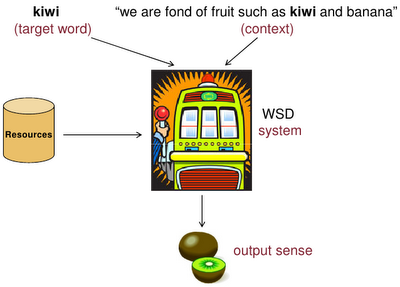
\includegraphics[scale=0.8]{wsd.png}
\caption{An example of word sense disambiguation system. Image courtesy ~\protect\cite{navilgiblog}}
\end{figure}

\subsection{Evaluation}
WSD systems are evaluated by comparing in terms of their coverage,precision and recall with respect to a gold tagging(gold tags are provided by human). We allow a empty sense assignment in case the system is not able to disambiguate the word. So for each word $w_i$ the output of the classifier lies in $S_i \cup \{\epsilon\}$. We can now define  our metrics as follows,
\begin{align*}
Precision = \frac{\text{\# of correct sense tags in the output}}{\text{Total \# of tags in the output}}\\
%Recall =\frac{\text{\# of correct sense tags in the output}}{\text{Total \# of tags in the gold tagging}}\\
%Coverage =\frac{\text{\# of tags in the output}}{\text{Total \# of correct tags in the gold tagging}}
\end{align*}
\subsection{The Data}
\label{sec:data}
%\instructions{Describe the data you use to train and evaluate your models. Describe where you got it from (include references/citations to published works, or URLs!). Describe and give examples for the features that you have access to.} 
We use datasets from \textbf{SemEval-2007}~\cite{semeval}. It is an ongoing series of evaluations of computational semantic analysis systems; it evolved from the Senseval word sense evaluation series. We choose a specific dataset from ``Task \# 7: Coarse-grained English all-words (Coarse AW)" to do both the training and testing. The chosen dataset contains coarse grained tags for approximately 6,000 words from five running texts. The coarse senses were based on a clustering of the WordNet sense inventory obtained via a mapping to the Oxford Dictionary of English (ODE), a long-established dictionary which encodes coarse sense distinctions. The dataset also contains the coarse-grained sense inventory which is prepared semi-automatically: starting from an automatic clustering of senses produced by~\cite{Navigli06} with the Structural Semantic Interconnections (SSI) algorithm, and then manually validate the clustering for the words occurring in the text. For each content word the dataset provides lemma and part of speech.

Our work also requires some libraries such as ``Wordnet" database and ``WS4J" library. We use the the latest released version for Wordnet 3.0 from~\cite{wordneturl}. We compute the similarity metrics by utilizing WS4J library from~\cite{WS4Jurl}.

\section{The Models}
\label{sec:models}

\subsection{Baseline Models}
\label{sec:baseline-models}
\begin{description}
\item[Random Baseline] A naive baseline for word sense disambiguation. A randomly selected sense is made from the set of permissible senses for the target word. \\
\item[First Sense Baseline (Most Frequent Sense)] A more appropriate baseline model will be to output the sense of the word which is most frequently encountered. On coarse grained senses, using this baseline gives an accuracy ranging from 50-60\%. As noted in~\cite{navigli2009word}, this baseline is often difficult to beat.
\end{description}
%
%\subsection{Existing Models}
%\label{sec:existing-models}
%\instructions{If people have worked on this task before, summarize (and cite) some of the existing models} 
%It-makes-sense
\subsection{Our Model}
\label{sec:proposed-models}
%\instructions{Your models and your procedure for learning them go here. Describe both in detail, even if the learning procedure is standard.}
We employ a graph-based approach to disambiguate senses of a word. Our method is similar to ~\cite{Sinha}. We define a fixed sized window around a target word in the document as its context. We first create a weighted graph of label dependencies for all candidate senses. For every candidate sense $s_{ij}$ for word $w_i$, we have a node in the graph. This node has edges to the all candidate senses of words within a pre-defined window around word $w_i$. These edges are weighed by the dependency score for the pair of senses. The dependency score captures the relationship between two candidate senses for nearby words. Based on the edge weights we assign scores to each node based on a graph-based measure of centrality. The score of a node denotes the "importance" of the node in the graph, taking into account its relationship with neighboring nodes.
Our method is different from~\cite{Sinha} in that we make use of the coarse grain senses provided in the Semeval corpus to construct our graph. Consequently, our graph is less dense than the graph constructed in~\cite{Sinha}.
\subsection{Measures of Centrality}
We use two measures of centrality - closeness and in-degree - for scoring the vertices in our graph. These were originally proposed in \cite{Sinha}. They are defined as follows, \\
\begin{align*} 
\text{closeness}(V)= \frac{1}{\sum\limits_{T \in Vertices}{\text{length of shortest path from V to T}}} \\
\text{in-degree}(V)= \sum\limits_{T \in Vertices} \text{there exists an edge from T to V} \\
\end{align*} 
\begin{figure}
\begin{algorithm}[H]
\SetKwInOut{Input}{input}
\SetKwInOut{Output}{output}
\Input{A document D and a list of ambiguous words $W=(w_1,w_2 \cdots w_n)$ such that $\forall i, w_i\in D$. \\
Each $w_i \in W$ admits a set of candidate senses $S_i=(s_{i1},s_{i2} \cdots s_{in_i})$ where $|S_i|= n_i$}
\Output{A graph G where a vertex represents a candidate sense of $w_i$ and has edges to candidate senses of $w_j$, $i\ne j$. The cost of the edge is determined by  a dependency scoring metric.}
\For{$word_1 \gets w_1$ \textbf{to} $w_n$}
{
	\For{$word_2 \gets w_1$ \textbf{to} $w_n$}
	{
		\If{$word_1.position - word_2.position>window_{max}$}
		{
			break
		}
		\Else
		{
			\For{$s_1 \in S_{word_1}$}
			{
				\For{$s_2 \in S_{word_2}$}
				{
					$vertex_1 \gets newVertex(s_1)$ \\
					$vertex_2 \gets newVertex(s_2)$ \\
					$edgeCost \gets getEdge(word_1,word_2,sense_1,sense_2,metric)$ 
					$addEdge(vertex_1,vertex_2,edgeCost)$
				}	
			}
		}
	}
}
\caption{Algorithm to generate the graph (adapted from~\cite{Sinha})}
\end{algorithm}
\begin{algorithm}[H]
\For{$word_i \gets w_1$ \textbf{to} $w_n$}
{
	$sense_i\gets \max\limits_{V_i \in S_i} score(V_i)$ \\
	where $S_i$ corresponds to possible senses of $word_i$ and $V_i$ is the respective vertex
}
\caption{Algorithm to assign Senses}
\end{algorithm}

\end{figure}

\section{Experiments}
\label{sec:experiments}

%\subsection{Experimental Hypotheses}
%\label{sec:exper-hypoth}
%\instructions{Summarize the hypotheses (research questions) your experiments are designed to test (address). (Note that some of these hypotheses may emerge as you keep working on a problem; you will not necessarily have come up with all the questions you wish to address before you have started building a models for the specific task.}

%\subsection{Experimental setup}
%\label{sec:experimental-setup}
%\instructions{Define test/training/dev data splits, describe how you tuned performance. Describe and your evaluation metric, and define it mathematically.
%List the models you will evaluate. Cite any existing tools or software you use to perform your experiments; describe what you implemented yourself. Describe how you obtained the features used by each of the models.}
%mention maven

\subsection{Experimental results}
\label{sec:experimental-results}
\begin{figure}
\centering
\begin{minipage}{.5\linewidth}
\begin{tabular}{|c|c|c|}
  & Lesk & LeacockChodrow & WuPalmer & Resnick & Lin  \\
\hline
Closeness & 73.56 & 63.77 & 64.17 & 68.66 & 67.12\\
Indegree & 80.34 & 80.34 & 80.34 & 80.34 & 80.34 \\
\end{tabular}
\caption{Precision of our system for different graph-centrality measures. We have reported the best performing systems for each measure, over all possible choices of similarity metric.}
\end{minipage}
\quad
\begin{tabular}{|c|c|c|c|c|c|}
POS & LeacockChodrow & Lesk & WuPalmer & Resnick & Lin  \\
\hline
Noun & 58.30 & 73.47 & 56.50& 67.78 & 62.18\\
Adjective & 86.19 & 85.36 & 86.19 & 86.19 & 86.19\\
Verb & 52.12 & 61.60 & 56.85 & 52.96 & 57.53\\
Adverb & 87.01 & 87.50 & 87.50 & 87.50 & 87.50\\
\end{tabular}
\caption{Precision for different part-of-speeches for each metric. The graph-centrality measure used for all results was closeness.}
\end{figure}
% BEGIN RECEIVE ORGTBL test
\begin{figure}
\begin{tabular}{|l|r|r|r|r|r|}
Metric & doc1 (368) & doc2 (379) & doc3 (345) & Doc4 (500) & Doc5 (677) \\
\hline
LeacockChodrow+closeness & 69.84 & 69.39 & 57.69 & 68.40 & 57.01 \\
Lesk+closeness & 83.42 & 83.64 & 62.60 & 75.40 & 66.77 \\
WuPalmer+closeness & 69.87 & 66.49 & 56.81 & 68.4 & 60.41 \\
Resnick+closeness & 77.99 & 77.30 & 58.84 & 65.2 & 66.32 \\
Lin+closeness & 72.55 & 76.25 & 54.50 & 61.40 & 69.71 \\
LeacockChodrow+indegree & 86.14 & 86.28 & 76.52 & 80.4 & 75.78 \\
Lesk+indegree & 86.14 & 86.28 & 76.52 & 80.4 & 75.78 \\
WuPalmer+indegree & 86.14 & 86.28 & 76.52 & 80.4 & 75.78 \\
Resnick+indegree & 86.14 & 86.28 & 76.52 & 80.4 & 75.78 \\
Lin+indegree & 86.14 & 86.28 & 76.52 & 80.4 & 75.78 \\
\end{tabular}
\caption{Document-wise precision for different combinations of metrics and graph-centrality measures. For each document, the total number of ambiguous words are shown in parenthesis.}
\end{figure}
% END RECEIVE ORGTBL test
\begin{comment}
#+ORGTBL: SEND test orgtbl-to-latex :splice nil :skip 0
| Metric                   | doc1 (368) | doc2 (379) | doc3 (345) | Doc4 (500) | Doc5 (677) |
| LeacockChodrow+closeness |      69.84 |      69.39 |      57.69 |      68.40 |      57.01 |
| Lesk+closeness           |      83.42 |      83.64 |      62.60 |      75.40 |      66.77 |
| WuPalmer+closeness       |      69.87 |      66.49 |      56.81 |       68.4 |      60.41 |
| Resnick+closeness        |      77.99 |      77.30 |      58.84 |       65.2 |      66.32 |
| Lin+closeness            |      72.55 |      76.25 |      54.50 |      61.40 |      69.71 |
| LeacockChodrow+indegree  |      86.14 |      86.28 |      76.52 |       80.4 |      75.78 |
| Lesk+indegree            |      86.14 |      86.28 |      76.52 |       80.4 |      75.78 |
| WuPalmer+indegree        |      86.14 |      86.28 |      76.52 |       80.4 |      75.78 |
| Resnick+indegree         |      86.14 |      86.28 |      76.52 |       80.4 |      75.78 |
| Lin+indegree             |      86.14 |      86.28 |      76.52 |       80.4 |      75.78 |
\end{comment}
% BEGIN RECEIVE ORGTBL results
\begin{figure}
\centering
\begin{tabular}{|l|r|}
System & Precision \\
\hline
NUS-PT & 82.50 \\
NUS-ML & 81.58 \\
LCC-WSD & 81.45 \\
\textbf{Our System} & \textbf{80.34}\\
GPLSI & 79.55 \\
Baseline & 78.89 \\
UPV-WSD & 78.63 \\
TKB-UO & 70.21 \\
PU-BCD & 69.72 \\
RACAI-SYNWSD & 65.71 \\
SUSSX-FR & 71.73 \\
USYD & 58.79 \\
UofL & 52.59 \\
SUSSX-C-WD & 54.54 \\
SUSSX-CR & 54.30 \\
\end{tabular}
\caption{Final Ranking for the SemEval-2007 Task. We have included our system in the list for comparison. The precision reported is for the best setting (using Lesk+In-Degree)}
\end{figure}
% END RECEIVE ORGTBL results
\begin{comment}
#+ORGTBL: SEND results orgtbl-to-latex :splice nil :skip 0
| System       | Precision |
| NUS-PT       |     82.50 |
| NUS-ML       |     81.58 |
| LCC-WSD      |     81.45 |
| GPLSI        |     79.55 |
| Baseline     |     78.89 |
| UPV-WSD      |     78.63 |
| TKB-UO       |     70.21 |
| PU-BCD       |     69.72 |
| RACAI-SYNWSD |     65.71 |
| SUSSX-FR     |     71.73 |
| USYD         |     58.79 |
| UofL         |     52.59 |
| SUSSX-C-WD   |     54.54 |
| SUSSX-CR     |     54.30 |
\end{comment}

\section{Conclusion}
From the experimental results we can infer that the baseline is actually hard to beat. This is also evident from the final rankings in the SemEval-2007 task, where many teams performed worse than the baseline. 
\section*{Your current to-do list}
\paragraph{Done}
\begin{enumerate}
\item Implemented the code.
\item Obtained the Semeval 2007 dataset.
\item Added relevant related work.
\end{enumerate}
\paragraph{Left to do}
\begin{enumerate}
\item Running experiments with different similarity metrics.
\item Write-up.
\end{enumerate}


\bibliographystyle{plain}
\bibliography{CS446projCheckIn}  
\end{document}
